\documentclass[a4paper,oneside,11pt]{report}
\usepackage{a4wide,graphicx,fancyhdr,amsmath,amssymb, standalone}

\usepackage{algpseudocode}
%-------- Macros and Definitions --------%

\setlength\headheight{20pt}
\addtolength\topmargin{-10pt}
\addtolength\footskip{20pt}

\newcommand{\subject}{2IO70 embedded systems}

\newcommand{\N}{\mathbb{N}}
\newcommand{\ch}{\mathcal{CH}}

\newcommand{\naam}{Reinhard Heinrich Bertram Vinzenz Freiherr von Pelden genannt Cloudt zu Lauersfort und Impel}

\fancypagestyle{plain}{%
\fancyhf{}
\fancyhead[LO,RE]{\sffamily\bfseries\large technische universiteit eindhoven}
\fancyhead[RO,LE]{\sffamily\bfseries\large \subject}
\fancyfoot[LO,RE]{\sffamily\bfseries\large department of mathematics and computer science}
\fancyfoot[RO,LE]{\sffamily\bfseries\thepage}
\renewcommand{\headrulewidth}{0pt}
\renewcommand{\footrulewidth}{0pt}
}

\pagestyle{fancy}
\fancyhf{}
\fancyhead[RO,LE]{\sffamily\bfseries\large technische universiteit eindhoven}
\fancyhead[LO,RE]{\sffamily\bfseries\large \subject}
\fancyfoot[LO,RE]{\sffamily\bfseries\large department of mathematics and computer science}
\fancyfoot[RO,LE]{\sffamily\bfseries\thepage}
\renewcommand{\headrulewidth}{1pt}
\renewcommand{\footrulewidth}{0pt}

\usepackage[margin=1in]{geometry}
\usepackage{float}
\usepackage{subcaption}
\usepackage{graphicx}

%-------- Title --------%

\title{\vspace{-\baselineskip}\sffamily\bfseries \Huge Final report 2IO70}
\author{
	\makebox[.25\linewidth]{Sergio van Amerongen}\\0952200 \and
	\makebox[.25\linewidth]{Stefan Cloudt}\\0940775 \and
	\makebox[.25\linewidth]{Daan de Graaf}\\0956112 \and
	\makebox[.25\linewidth]{Robert van Lente}\\0953343 \and
	\makebox[.25\linewidth]{Tom Peters}\\0948730 \and
	\makebox[.25\linewidth]{Berrie Trippe}\\0948147 
	\and \makebox[.75\linewidth]{\textbf{Responsible:}} \and
	Daan de Graaf\\ \tt{d.j.a.d.graaf@student.tue.nl}
}
\date{\today}

%-------- Document --------%

\begin{document}
\maketitle

\tableofcontents

\chapter{Introduction}
\textit{
On an Easter morning, you are rudely woken by the merciless beeping of your alarm clock. In a reflex, you grab your phone from the nightstand to check up on your social media. You catch a glimpse of the time on your phone, and cry out in horror as you realise that your alarm clock does not account for daylight savings. Fueled by adrenalin you sprint downstairs, and are subsequently greeted by the smell of fresh coffee, which your coffee machine is programmed to make you every day. You resist your craving for caffeine and enter your car. You enter your sister's new address on your satellite navigation and drive off in silence, as your little one recently discovered the disc drive slot on the car stereo and decided it would make an ideal place to dispose of chewing gum. As much as that confused the car stereo, your GPS system is equally bewildered to find you taking a right turn where you should only have gone slightly right.
}
\\\\
Nowadays, embedded systems are ubiquitous. They make sure you awake in time, satisfy your caffeine addiction and guide you from A to B. These devices all work flawlessly, were it not for one misbehaving part: Us. These machines have to work with our complicated time zones and daylight savings, deal with improper usage and even know the things we forget to tell them in order to do their jobs right! Surely, we can not expect any machine to account for all of this? Therefore, the best we can do is make machines as fault-tolerant as possible, and clearly communicate with the user when something inevitably goes wrong.

This project is about sorting black and white discs. The machine made in this project is not only able to sort, but it can also detect errors during its process and give an adequate response. The machine is therefore able to tell something about its operating state, which is considered difficult.


\chapter{Machine design}
\documentclass[a4paper,oneside,11pt]{article}
\usepackage{a4wide,graphicx,fancyhdr,amsmath,amssymb}

%-------- Macros and Definitions --------%

\setlength\headheight{20pt}
\addtolength\topmargin{-10pt}
\addtolength\footskip{20pt}

\newcommand{\subject}{2IO70 embedded systems}

\newcommand{\N}{\mathbb{N}}
\newcommand{\ch}{\mathcal{CH}}

\newcommand{\naam}{Reinhard Heinrich Bertram Vinzenz Freiherr von Pelden genannt Cloudt zu Lauersfort und Impel}

\fancypagestyle{plain}{%
\fancyhf{}
\fancyhead[LO,RE]{\sffamily\bfseries\large technische universiteit eindhoven}
\fancyhead[RO,LE]{\sffamily\bfseries\large \subject}
\fancyfoot[LO,RE]{\sffamily\bfseries\large department of mathematics and computer science}
\fancyfoot[RO,LE]{\sffamily\bfseries\thepage}
\renewcommand{\headrulewidth}{0pt}
\renewcommand{\footrulewidth}{0pt}
}

\pagestyle{fancy}
\fancyhf{}
\fancyhead[RO,LE]{\sffamily\bfseries\large technische universiteit eindhoven}
\fancyhead[LO,RE]{\sffamily\bfseries\large \subject}
\fancyfoot[LO,RE]{\sffamily\bfseries\large department of mathematics and computer science}
\fancyfoot[RO,LE]{\sffamily\bfseries\thepage}
\renewcommand{\headrulewidth}{1pt}
\renewcommand{\footrulewidth}{0pt}

\usepackage[margin=1in]{geometry}
\usepackage{float}
\usepackage{subcaption}
\usepackage{graphicx}

%-------- Title --------%

\title{\vspace{-\baselineskip}\sffamily\bfseries Machine Design}
\author{
	\makebox[.25\linewidth]{Sergio van Amerongen}\\0952200 \and
	\makebox[.25\linewidth]{Stefan Cloudt}\\0940775 \and
	\makebox[.25\linewidth]{Daan de Graaf}\\0956112 \and
	\makebox[.25\linewidth]{Robert van Lente}\\0953343 \and
	\makebox[.25\linewidth]{Tom Peters}\\0948730 \and
	\makebox[.25\linewidth]{Berrie Trippe}\\0948147 
	\and \makebox[.75\linewidth]{\textbf{Responsible:}} \and
	Robert van Lente\\ \tt{r.f.v.lente@student.tue.nl}
}
\date{\today}

%-------- Document --------%

\begin{document}
\maketitle

\section{Introduction}
We started our project by determining the features that we wanted to implement in our sorting machine, like user interaction and exception handling. These design decisions form the foundation of our mechanical machine design. The purpose of this document is to record the design decisions we made in the first stage of the project, from a mechanical point of view as well as
a user point of view.

\section{Design requirements}
In order to create a functioning sorting machine that can sort black and white discs, at least the following components are required.
\begin{itemize}
\item A container for storing unsorted discs
\item Two containers for storing the sorted discs
\item A sensor that can distinguish the different colour discs.
\item A transporter that is able to move the discs from the container to the sensor.
\item A transporter that is able to move the discs from the sensor to the appropriate container.
\end{itemize}

\section{Final Design}
The machine consists of a vertical tube in which the discs can be stored. A pin can be removed from the bottom of the tube, allowing the discs to fall on a platform below, one by one. A colour sensor is attached underneath this platform, such that it can detect the colour of the disc.
Next to this platform, a step motor is attached that rotates a wheel with three arms. These arms can push the disc of the platform, either on the left or the right side.
Below the platform, a seesaw is attached with both sides of the same length, such that the discs that fall on the platform can fall on these arms. A gyroscope is attached to the axis of this seesaw, such that rotations of the seesaw can be detected.
The discs then slide off the seesaw, allowing it to stabilize, and fall into one of two mountable trays.

\section{Design Decisions}
The machine went through several iterations before we settled on the final design. Below the decisions that we made during the design process are listed.

\subsection{Position of the colour sensor}
We had the option to attach the colour sensor in various ways to the machine. We chose to put it underneath the platform with the sensor pointing up, in such way that the arm of the motor could easily wipe the discs away.  Placing the sensor below the discs makes the sensor more reliable, since the surface of the discs on the bottom is larger than the surface on the side of the discs. It would also have been significantly more difficult to mount the colour sensor in a sideways or upright position because of the structural limitations of the construction set.

\subsection{Container}
The decision to use a tube-like structure was made early on, as it is the most compact way to store the discs. The vertical storage also has the added benefit of removing the need to create an additional transporter to move the discs from the container to the sensor, since a new disc will simply fall in place when the previous disc is moved away.

The height between the tube and the platform is designed to be slightly higher than the height of one disc. This ensures that only one disc will be moved from the tube at the time.

\subsection{Rotating arm}
The wheel to which the arms are attached are used to transport the discs from the sensor to the trays. We had options to put 3 or 4 arms on the wheel. We chose to go for 3 arms because then we would be able to attach a touch sensor which is used for calibration.

\subsection{Seesaw}
Initially, the plan was to use touch sensors to detect if a disc arrived in the correct tray. However, we quickly found that the discs did not weigh enough to trigger the touch sensors. Therefore we settled finally with the seesaw and a gyroscope attached to it.

\subsection{Trays}
We chose to use coffee cups for the trays in the machine, since these where readily and freely available. Other options would be buying plastic trays or building trays out of LEGO, which was not possible because there was not a sufficient number of parts in the construction set.

\begin{figure}[H]
\begin{subfigure}{0.5\textwidth}
	\centering
	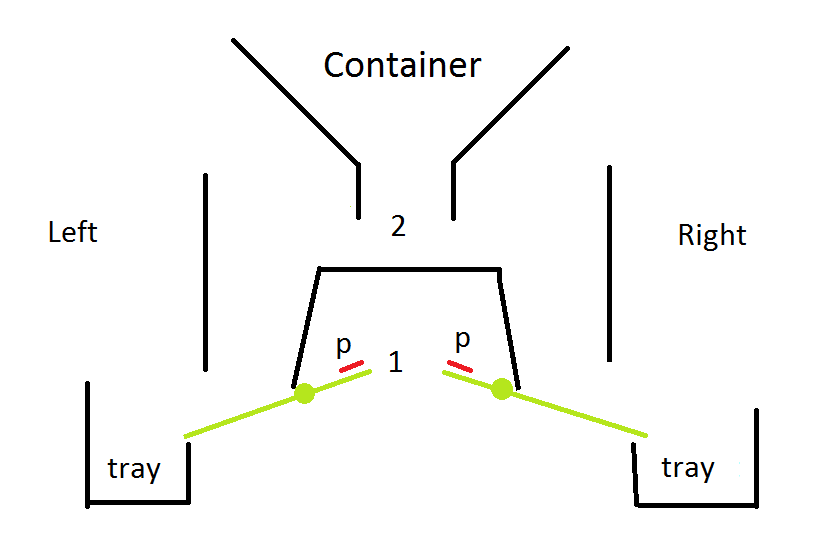
\includegraphics[width=80mm]{front}
	\caption{\label{firstfront}Front view}	
\end{subfigure}	
\begin{subfigure}{0.5\textwidth}
\centering
	\includegraphics[width=80mm]{top}
	\caption{\label{top}Top view.}
\end{subfigure}	
\caption{The initial design of the machine.}
\end{figure}

\begin{figure}[H]
	\centering
	\includegraphics[width=90mm]{frontnew}
	\caption{\label{front}The final front view of the machine.}
\end{figure}

\section{System Level Requirements}
\subsection{Use Cases}
The machine can be described as a finite automaton. This finite automaton is shown in figure
3. The machine has three buttons, which the user can utilize to control the machine. The
START/PAUSE button is used to start and pause the machine. The ABORT button is used to
stop the machine in case of emergency. The RESET button is used to reset the machine. The
user is required to add black or white discs to the container before starting the machine.
The machine, when finished without fatal error, produces two trays, one filled with white
and one filled with black discs. The machine will also display information about its current
state and progress on the display during the sorting process.

The sorting process is described by the following automaton. The initial state is the rest-
ing state. The user is required to prepare the machine as described in the User Constraints segment further in the document. None of the buttons should have any effect, except for the
START/PAUSE button. When this button is pressed, the machine should proceed to the
operating state.

In this state, the machine sorts the discs. Internally, it has a state in which it checks the
color of the disc, after which it moves to the correct sorting state in which it transports the disc
to the correct tray. If the RESET button is pressed in this state, the machine should return to
the resting state.

While in the operating state, if the START/PAUSE is pressed, the process should halt
and the machine should go into a paused state. When the START/PAUSE button is pressed
again, the machine should return to the operating state at the point where it was when the
START/PAUSE button was first pressed. If the RESET button is pressed in this pausing state,
the machine should return to the resting state.

While in the operating state, if the ABORT button is pressed or a fatal exception is encoun-
tered, the machine should immediately go into an exception state. In this state, the machine
must come to a full stop. The machine should only continue when the RESET button is pressed,
after which it returns to the resting state.

When the machine finds that there are no more discs left in the storage, it should go into a
finished state. Then, if the RESET button is pressed, the machine should return to the resting
State.

\begin{figure}[H]
	\centering
	\includegraphics[width=125mm]{machinedesign}
	\caption{\label{machinedesign}The finite state automaton of the machine.}
\end{figure}

\subsection{User Constraints}
\subsubsection{Machine Preparation}
Machine Preparation Before starting the operation of the machine with the START/PAUSE
button in the resting state, the user is expected to fill the disc storage device with black and
white colored discs that need to be sorted. Only discs are allowed in the disc storage and no
other objects should be placed in it. The user must also ensure that no discs are present in
other parts of the machine and that the disc trays are mounted to their mounting points prior
to starting execution. The disc trays should be empty. At most 12 discs may place into the
container. The user then has to proceed by starting the program. The tube can be filled with
discs after the machine has finished calibrating the moving arm.

After the machine has finished execution, the user will have access to two trays, one containing exclusively white discs, the other only contains black discs. When the machine indicates
that it has finished its sorting procedure, the user should remove the trays from their mounts
so he can dispose the discs somewhere else.

\subsubsection{Exceptions}
Possible errors are as follows:
\begin{figure}[H]
\centering
\begin{tabular}{|l|l|}
\hline
Error type & Fatal (= go to abort state)\\\hline
Disc does not reach the tray & Yes\\\hline
Disc arrives in the wrong tray & No\\\hline
Time to tray is higher than average & No\\\hline
Wrong input (i.e. different colour disc) & No\\\hline
Motor jams & Yes \\\hline
Gyroscope does not stabilise & Yes \\\hline
%Connection to peripheral lost & Yes \\\hline
Battery low & Yes \\\hline
Abort by user & Yes \\\hline
Software exception & Yes \\\hline
\end{tabular}
\end{figure}
When a disc does not reach the tray, the machine should stop, as there is may be an
obstruction in the path the disc takes from the sorting arm to the lever.

When a disc arrives in the wrong tray, the machine should stop, as something happened
that caused the disc to move to the wrong tray, even though the sorting arm tried to move
it to the correct tray. This means there must be a mechanical failure somewhere.

The Wrong Input error occurs when a disc is being detected with another color than white
or black. This could, for example, be a disc with the color red. This is not a fatal error because
we can specify an action that will be taken when this exception occurs. We may for example
want the machine to simply put the unknown disc in one of the trays anyway, say default the
destination to white, or we dispose all unknown discs into a separate tray.

%The connection to peripherals lost exception is marked as a fatal exception, because a defect
%in the controlling parts of the machine prevent it from functioning properly for obvious reasons.
%The user has to fix this by hand before the machine can be used again.

The machine will stop operation when the battery has less than 5% of charge left. This
is done to prevent the machine running out of power in between operations and ending in an
invalid state.

When an error occurs in the machine that is indicated with fatal, the user must remove all
discs from all parts of the machine. The user should then press the RESET button in order
to put the machine in its resting state. The user may then proceed to prepare the machine for
execution again, as described above, if desired.

\paragraph{Safety properties}
The machine should have the following safety properties. These are our
guarantees about the working and stopping conditions of the machine, in case something unex-
pected happens.

\begin{itemize}
	\item The ABORT button must stop all moving parts within 10 ms. This to make sure that the user is able to quickly stop the machine in case something can not be handled by the Machine.
	\item When the machine starts with discs loaded into the container, then the discs will be sorted
when it arrives in the finished state. The sorting process takes at most 5 minutes in the
default safe mode. However software specification may specify more modes.
	\item A fatal exception must stop all moving parts within 10 ms. This ensures that the machine
does not damage or even destroy itself when it is blocked in any way.
\end{itemize}

\section{Machine Interface}
\subsection{Lejos API}
The Lejos API provides access to buttons on the brick, sensors and actuators.
Buttons can be queried directly, but references to sensors and actuators must be instantiated
with a ’Port’ parameter indicating how they are connected to the brick. The following ports
are used in our design:

\begin{figure}[H]
\begin{tabular}{|l|l|}
\hline
\textbf{Peripheral} & \textbf{Port} \\
\hline
Colour sensor & Port 1 \\
Gyroscope & Port 2 \\
Touch sensor & Port 3 \\
Motor & Port A \\
\hline
\end{tabular}
\end{figure}

Motors expose methods that allow the developer to have to motor rotate an arbitrary number of degrees. Therefore, it is not necessary to implement pulse width modulation. One can call a method to fetch a sample from a sensor in the form of an array of floats. It is up to the developer to parse these in a meaningful way.

\subsection{Peripherals}

\subsubsection{Motor rotating arm}
This motor is connected to port A and rotates the arm which moves the discs. The arm has three legs with an angle of 120 degrees. The motor has basically three states: a resting state and two working states, one for every possible direction. The neutral position of the three legged arm is the position where the two arms closest to the place where the disc will land have an approximately identical distance to the disc. When the motor is in the resting state the three legged wheel has this neutral position. When the motor is in a working state the arms rotate left or right until the next neutral position of the wheel (120 degrees further), where it will transition to the resting state of the motor. During the working state the motor should not be jammed or obstructed in any way, or the motor will be jammed and trigger an exception.

When the motor is in a working state the arms rotate left or right until the next neutral position of the wheel (120 degrees further), where it will transition to the resting state of the motor. During the working state the motor should not be jammed or obstructed in any way, or the motor will be jammed and trigger an exception.

\subsubsection{Touch sensor calibrator}
The touch sensor, connected to port 3, is attached in such a way behind the sorting platform that the arms of the sorting wheel are able to fully press the sensor when it rotates. This way, it is possible to detect the position of the sorting wheel when it is rotating, which can be used to calibrate the sorting wheel through software.

\subsubsection{Gyroscope with seesaw}
To the seesaw a gyroscope is attached, which is wired to port 2. The seesaw has three states, a neutral state, a left-side down state and a right-side down state. The neutral state is the state in which the gyroscope when read returns a value indicating that it is in balance. The seesaw enters a left-side down state when a disc falls on the left side. The gyroscope will read a value indicating that it was unbalanced and that the left side went down.
This is analogous for the right side down state.

\subsubsection{Colour sensor}
The colour sensor, connected to port 1, gives a value indicating the colour of the surface above it. The colour sensor returns an integer indicating the colour of the disc (e.g. 0 for red, 1 for green etc.) currently on the platform, or -1 if only ambient light was reaches the detector, indicating that there is no disc on the platform. The sensor is able to distinguish 15 different colours, as shown in the following table:

\begin{figure}[H]
\begin{tabular}{|l|l|}
\hline
\textbf{Colour} & \textbf{Value} \\
\hline
None & -1 \\
Red & 0 \\
Green & 1 \\
Blue & 2 \\
Yellow & 3 \\
Magenta & 4 \\
Orange & 5 \\
White & 6 \\
Black & 7 \\
Pink & 8 \\
Gray & 9 \\
Light Gray & 10 \\
Dark Gray & 11 \\
Cyan & 12 \\
Brown & 13 \\
\hline
\end{tabular}
\end{figure}

\subsubsection{The brick}
The brick controls the sensors and actuators. The state of the buttons is either
up or down, which may be queried using the Lejos API. The buttons used are shown in figure \ref{brickbuttons}.
\begin{figure}[H]
	\centering
	\includegraphics[width=60mm]{BrickButtons}
	\caption{\label{brickbuttons}The buttons on the brick.}
\end{figure}

\section{Conclusion}
The design decisions recorded in this document will be built upon in the next phase of the
project, where we are going to specify the software specifications. The software specifications
are heavily dependent on the machine interface described in this document, since the machine
interface describe our assumptions about the machine API and the mechanical implementation.
The software specifications will describe how we are going to use this interface and how the
machine will behave.

\section{Sources}
\begin{description}
\item[Colour table]  http://www.lejos.org/ev3/docs/ - Constant Field Values
\end{description}
\end{document}


\chapter {Software specification}
\documentclass[a4paper,oneside,11pt]{article}
\usepackage{a4wide,graphicx,fancyhdr,amsmath,amssymb}

%-------- Macros and Definitions --------%

\setlength\headheight{20pt}
\addtolength\topmargin{-10pt}
\addtolength\footskip{20pt}

\newcommand{\subject}{2IO70 embedded systems}

\newcommand{\N}{\mathbb{N}}
\newcommand{\ch}{\mathcal{CH}}

\newcommand{\naam}{Reinhard Heinrich Bertram Vinzenz Freiherr von Pelden genannt Cloudt zu Lauersfort und Impel}

\fancypagestyle{plain}{%
\fancyhf{}
\fancyhead[LO,RE]{\sffamily\bfseries\large technische universiteit eindhoven}
\fancyhead[RO,LE]{\sffamily\bfseries\large \subject}
\fancyfoot[LO,RE]{\sffamily\bfseries\large department of mathematics and computer science}
\fancyfoot[RO,LE]{\sffamily\bfseries\thepage}
\renewcommand{\headrulewidth}{0pt}
\renewcommand{\footrulewidth}{0pt}
}

\pagestyle{fancy}
\fancyhf{}
\fancyhead[RO,LE]{\sffamily\bfseries\large technische universiteit eindhoven}
\fancyhead[LO,RE]{\sffamily\bfseries\large \subject}
\fancyfoot[LO,RE]{\sffamily\bfseries\large department of mathematics and computer science}
\fancyfoot[RO,LE]{\sffamily\bfseries\thepage}
\renewcommand{\headrulewidth}{1pt}
\renewcommand{\footrulewidth}{0pt}

\usepackage[margin=1in]{geometry}
\usepackage{float}
\usepackage{subcaption}
\usepackage{graphicx}

%-------- Title --------%

\title{\vspace{-\baselineskip}\sffamily\bfseries Software Specification}
\author{
	\makebox[.25\linewidth]{Sergio van Amerongen}\\0952200 \and
	\makebox[.25\linewidth]{Stefan Cloudt}\\0940775 \and
	\makebox[.25\linewidth]{Daan de Graaf}\\0956112 \and
	\makebox[.25\linewidth]{Robert van Lente}\\0953343 \and
	\makebox[.25\linewidth]{Tom Peters}\\0948730 \and
	\makebox[.25\linewidth]{Berrie Trippe}\\0948147 
	\and \makebox[.75\linewidth]{\textbf{Responsible:}} \and
	Tom Peters\\ \tt{t.peters@student.tue.nl}
}
\date{\today}

%-------- Document --------%

\begin{document}
\maketitle

\section{Introduction}
After having designed the machine, we are able to specify how our software should behave. We do this by describing the software in a state machine with abstract states. This state machine also implements the different operation modes. After this we characterise the distinct inputs and outputs. We will convert the state diagram into a working UPPAAL model and explain its different systems in detail. Finally we explain the verification of our model.

\section{Operation modes}
The gyroscope can be quite a bottleneck in the sorting process, as it is rather slow. If we want to sort very fast, we should skip the input from the gyroscope and sort the discs immediately after each other. Therefore, we want to implement 2 modes: a fast mode in which we do not check for input from the gyroscope and thus do not check if the disc actually reaches the tray, and a slower safe mode, where we check for input from the gyroscope and we can make sure that discs do reach the tray. Besides this, we want to make an additional incremental mode for debug purposes, in which the user has to press a button for the machine to sort the next disc.

\subsection{Fast mode}
This mode can be accessed by pressing the left button during mode selection. The machine starts in a resting state. If the left button is pressed in this state, the machine should go to the read color state. In this state, the machine checks which color disc is present on top of the light sensor. There are four different transitions the machine can make at this point, depended on the detected colour. If the machine is black or white, it should go to a respective state in which the motor is rotated accordingly. When the motor has finished moving, the machine simply returns to the read color state and repeats the process until no more discs are detected. The user should be able to pause the machine by pressing the START/PAUSE button anytime during the sorting process. The machine should then go to a paused state as soon as it enters the read color state and wait for a press of the START/PAUSE button again to continue the checking process. The user should also be able to abort the machine at any time using the ABORT button and reset it afterwards to let the machine return to the mode selection state.

\newpage

\subsection{Safe mode}
This mode can be accessed by pressing the middle button during mode selection. The safe mode is operates similarly to the fast mode, with some additional safety checks. After the motor has finished turning, the machine should enter a state in which it waits for input from the gyroscope to confirm that the disc arrived in the correct tray. Based on this input, the machine should be able to detect most errors described in Machine Design. 

\subsection{Incremental mode}
This mode can be accessed by pressing the right button during mode selection. The incremental mode is very similar to the safe mode. The difference is that the machine should go to a seperate state when it is finished sorting a single disc. In this state, the machine waits for a press on the START/STOP button to continue. Then, it simply continues the sorting process.

\subsection{Colour sensor calibration}
This feature can be accessed by pressing the up button during mode selection. Before accessing this state, the user should put a black disc and a white disc in the machine in that order. The rest of the tube should be left empty and tilted upwards. When this mode is entered, the colour sensor reads the values of a black disc, a white disc and nothing and saves them to use these values later in a sorting process.

\subsection{Exit}
By pressing the down button during mode selection, the program quits.

\section{Signals}
\subsection{Inputs:}
\subsubsection{Color c:} The input from the sensor with the following possible values: "N", "W", "B" and "U". The value "N" implies that no disk has been detected in front of the colour sensor. The value "W" implies that a white coloured disk is in front of the sensor. The value "B" implies that a black disk is in front of the sensor. Finally a value "U" means that an unknown disc is in front of the sensor.
\subsubsection{Motor M:} The input from the motor can be that it is jammed, “J”, or that it is finished, “F”. We use these inputs as a method to detect if we can go to the next state, or to detect if there is a possible error.
\subsubsection{Abort A:} This signal is high when the abort button has been pressed. This signal indicates that the machine should be halted nearly instantaneously and that the machine should enter the Abort state.
\subsubsection{Reset R:} This signal is high when the Reset button is pressed. The signal will be used to bring the machine back in its resting state and reset all the statistics about the current sorting operation.
\subsubsection{Start/Pause S/P:} This signal is high when the Start/Pause button is pressed. This signal will be used to start and pause the operation of the machine, depending on its current state.
\paragraph{Gyroscope G:} This signal might have three values "L", "R" and "S". "L" indicates that gyroscope is left, "R" indicates that the gyroscope is right and "S" indicates that the gyroscope is stable.

\subsection{Outputs}
\subsubsection{Colour Sensor CS:} Whether the colour sensor is currently reading the sensor values. In order to read the values, a light from within the sensor has to be activated in order for the detection to work. This means that this light is an output for the machine. While the light is activated, the sensor is constantly reading the sensor values, but we only read it in certain situations. The colour sensor is only active while the machine is in the operating state and is therefore disabled in the Resting state, Abort state, Finished state and the Paused state.
\subsubsection{Motor M:} This signal has three possible values "L", "R" and "O". Where "L" is the motor moving to the left for 120 degrees, "R" is the motor moving to the right for 120 degrees, "O" is the motor turned off. The sorting arm moves, depending on the colour read.
\subsubsection{LED Active E:} The EV3 controller brick has a built-in LED behind the buttons that we can use to give feedback to the user. We can specify the flashing pattern from a limited set of patterns and we can specify the colour. The LED will emit a constant green colour while the machine is in the Finished state. The LED will flash in red while it is in the Abort state. The LED will flash orange when it is in a warning state.
\subsubsection{Sound:} The brick also features a built-in speaker which we can use to give even more feedback to the user. We will use this speaker to let the user now what happens in the machine. So when there is an error, the machine will sound an error. When the machine finishes sorting it will play tiroler music.

\section{State Machine}
\begin{figure}[H]
	\centering
	\includegraphics[width=140mm]{statemachine}
	\caption{This state machine defines the behaviour of the software. The three modes of our machine have been embedded into the figure. Black coloured transitions are done in all modes.}
\end{figure}
We have indicated the transitions for specific modes using a colour coding. Green transitions only apply to the fast mode. Red transitions only apply to the incremental mode. Blue transitions only apply to the safe mode. 

All symbols are inputs or outputs defined in the previous chapter. However some symbols are not input or output but something else, these are documented here:

\begin{figure}[H]
\begin{tabular}{|l|l|}
\hline
\textbf{Symbol} & \textbf{Description} \\
\hline
PS & Starts the peripherals in order to be able to use them. This means setting output CS \\
 &  to active and M=O \\
PR & Resets the peripherals to turn them off, sets the CS to non active and M=O \\
TS & Starts a timer which increments variable $t$ at a fixed time rate \\
TR & Resets the timer by setting $t$ to 0\\
$t$ & The variable containing the current timer value \\
$tdmax$ & The maximum timer value after which it is decided that a disk was lost \\
$tavg$ & The average time of a disk to get in the basket \\
$tgmax$ & The maximum time it should take to stabilize the gyroscope \\
$paused$ & Variable indicating if the machine should go into the paused state or not \\
$reset$ & Variable indicating if the machine should go into the reset state or not \\
\hline
\end{tabular}
\end{figure}

\section{UPPAAL model}
An UPPAAL model consist of multiple systems that communicate over several channels. The systems in our UPPAAL model are Reinhard, our main system, along with several other peripheral systems.

\begin{figure}[H]
	\centering
	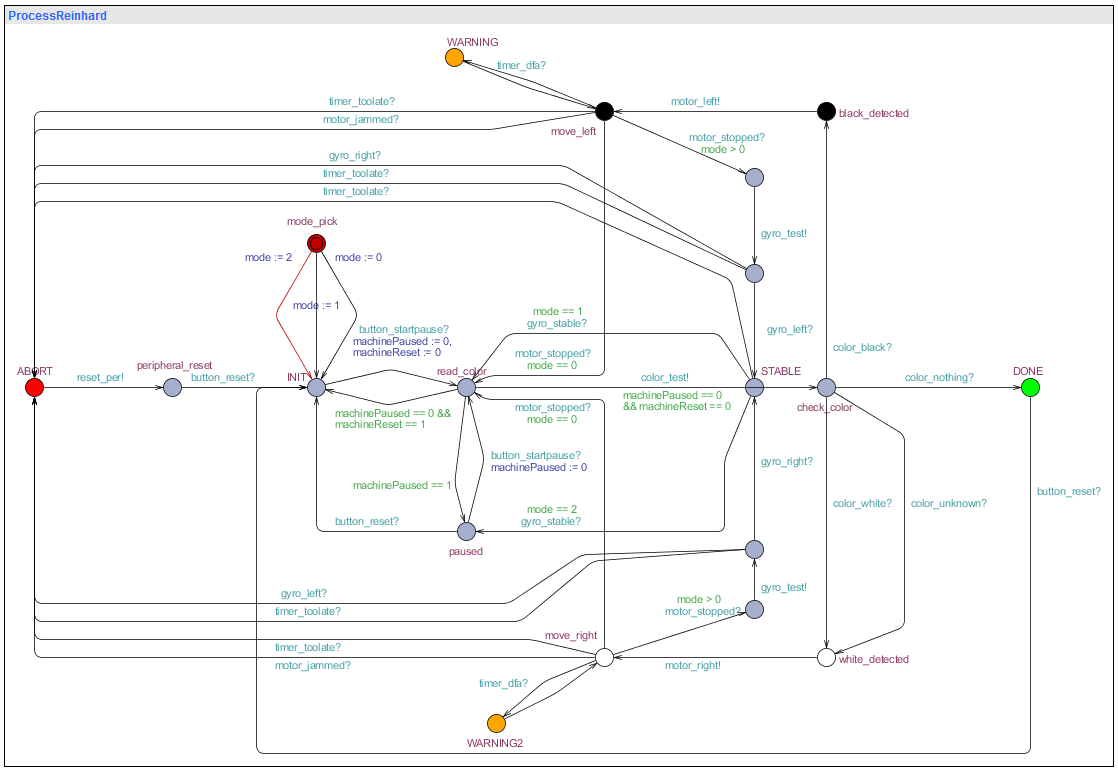
\includegraphics[width=150mm]{mainprocess}
	\caption{The main process in the UPPAAL model.}
\end{figure}

\subsection{Main process}
\subsubsection{Choosing the mode}
The initial state is mode\_pick. In this mode one of the three operation modes is chosen. This is important for the verification process, because the UPPAAL model uses an internal variable to store the mode, whereas the state machine indicates the different modes with colours. If it is not possible to set this variable in the model itself, the verification process will only verify if a query holds for one mode.

\subsubsection{Initialiation}
Upon choosing a mode, we enter the state INIT, which is equivalent to the initial state in the state machine. Here, the model waits for the button\_startpause signal from ProcessButtons. When the signal is received, it sets the machinePaused and machineReset variable to 0, which ensures that the model does not immediately pause or reset and moves to the next state.

\subsubsection{Reading colours}
Upon leaving the INIT state we enter the read\_color state (read in the state machine). Whenever the machinePaused variable is 1 in the read\_color state, the model goes to the paused state. If the machineReset variable is 1, the machine returns to the mode\_pick state, but this has the lower priority. If both of these are 0, the color\_test signal is send and the model transitions to the check\_color state.  In the check\_color state it waits for a signal of the ColorSensor system depending on whether there is a disc and which colour the disc has. Depending on the colour, it goes to one of two parts of the main system, one for each distinct colour (black or white). We will describe one of these parts as they are mirrored. Upon receiving the signal of a colour, the model transitions to a detected state. Here, it sends a signal to ProcessMotor to start moving in the appropriate direction and goes into a move state. The transition the model makes here is dependent on the mode variable.

\subsubsection{Check sequence}
If mode is not 0, indicating that the system is in the safe or incremental mode, it will add a check sequence using the gyroscope. After the signal from the motor is received that it has stopped, the main system will send a test signal to the GyroSensor waiting for a signal back. If the correct signal is received back, indicating that the disc has arrived in the correct tray, it will return to read\_color state. If mode is 0, indicating that the system is in fast mode, this check is skipped and the model returns to the read\_color state from the move state as soon as it receives the motor\_stopped signal from ProcessMotor.

\subsubsection{Finishing up}
When the model receives the color\_nothing signal from ProcessColorSensor, the machine is finished and the model goes to the DONE state. Here it waits for the button\_reset signal and returns to the initial state.

\subsubsection{Exceptions}
In our machine design is it specified that there is an ABORT button present that will stop the whole machine almost immediately. However, we have chosen not to include the abort button in our UPPAAL model as a possible transition for every state because this would be rather cumbersome and just a small implementation. We have however chosen to include the relevant exceptions specified in Machine Design. These transitions will lead the system into the ABORT state. In this state the process waits for the reset button to give a signal, after which it will reset the other processes and return to the initial state. Note that it is not required to actually reset the gyroscope in the actual machine, just in the UPPAAL model. Non-fatal exceptions are also represented in the model. Deviating average detection time is represented in the states WARNING and WARNING2, which the model reaches when the timer\_dfa is send from ProcessTimer. These warning states simply return to the state they were detected in and let the model continue.

\subsection{Subprocesses}
The following are all subprocesses that the main process depends on:

\subsubsection{ProcessColorSensor} waits for the $color\_test$ signal. It can then send four different signals: $color\_black$, $color\_white$, $color\_unknown$, and $color\_nothing$.

\subsubsection{ProcessMotor} waits for the $motor\_left$ or $motor\_right$ signal and moves to the respective state. From there, it can send either a $motor\_stopped$ or a $motor\_jammed$ signal. It also listens for a $reset\_per$ signal, after which it returns to the initial state.

\subsubsection{ProcessGyroSensor} waits for the $gyro\_test$ signal from the main process. It can then send the following signals: $gyro\_stable$, $gyro\_left$ and $gyro\_right$. If either $gyro\_left$ or $gyro\_right$ is send, the machine goes to an additional state where it is able to send a $gyro\_stable$ signal, indicating that the gyroscope has returned to its initial position. The process also listens for the $reset\_per$ signal, for resetting purposes.

\subsubsection{ProcessButtons} is continuously able to send button signals. This simulates that any button can be pressed at any time, which is necessary for the verifier to check all possible transitions. 

\subsubsection{ProcessTimer} works the same as ProcessButtons, but with signals that an internal timer would send if it detected one of the errors.

\subsubsection{ProcessPauseListener} and \textbf{ProcessResetListener} continuously listen to the $button\_startpause$ and $button\_reset$ signals from ProcessButtons. When they detect the respective signals, they set the respective variables to 1 to alert the main process that the button is pressed.

\begin{figure}[H]
\centering
\begin{subfigure}{0.1\textwidth}
\centering
\includegraphics[height=50mm]{processcolorsensor}
\caption{Colour sensor}
\end{subfigure}
\hfill
\begin{subfigure}{0.3\textwidth}
\centering
\includegraphics[height=50mm]{processmotor}
\caption{Motor}
\end{subfigure}
\hfill
\begin{subfigure}{0.3\textwidth}
\centering
\includegraphics[height=50mm]{processgyrosensor}
\caption{Gyroscope}
\end{subfigure}

\begin{subfigure}{0.45\textwidth}
\centering
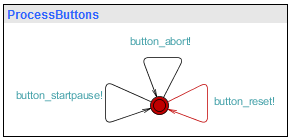
\includegraphics[height=30mm]{processbuttons}
\caption{Buttons}
\end{subfigure}
\hfill
\begin{subfigure}{0.45\textwidth}
\centering
\includegraphics[height=30mm]{processtimer}
\caption{Colour sensor}
\end{subfigure}

\begin{subfigure}{0.45\textwidth}
\centering
\includegraphics[height=40mm]{processpauselistener}
\caption{Pause listener}
\end{subfigure}
\hfill
\begin{subfigure}{0.45\textwidth}
\centering
\includegraphics[height=40mm]{processresetlistener}
\caption{Reset listener}
\end{subfigure}
\caption{Subprocesses}
\end{figure}

\section{Verification}
The main reason for recreating the state machine in UPPAAL was to allow extensive verification of the model. With UPPAAL we can verify whether certain queries hold for our model. The UPPAAL query language is a minimalistic but functional language to specify these properties. We use the following queries to verify our model:

\subsection{No deadlock}
Query: A[] not deadlock \\
Description: The system never deadlocks in any case \\
The machine will never stop responding to input.

\subsection{Valid mode specified}
Query: A[] mode==0 or mode==1 or mode==2 \\
Description: Mode must be one of: full speed, safe or incremental. \\
The mode value must be valid.

\subsection{DONE state reachability}
Query: E$<>$ ProcessReinhard.DONE \\
Description: There exists a path where the system reaches the ABORT state \\
This check ensures that the machine can eventually finish the sorting process.

\subsection{ABORT state reachability}
Query: E$<>$ ProcessReinhard.ABORT \\
Description: There exists a path where the system reaches the ABORT state.\\
We want to ensure that the machine halts in case of a fatal error. This check ensures that it is theoretically possible for a fatal error to occur and jump to the ABORT state.

\subsection{ABORT state avoidability}
Query: E[] not ProcessReinhard.ABORT \\
Description: There exists a path where the system does not reach the ABORT state.\\
We want to ensure that the machine is capable of running correctly without encountering fatal errors. This check ensures that it is possible to complete the sorting process error-free.

\subsection{Peripheral reset}
Query: A[] (ProcessReinhard.paused or ProcessReinhard.INIT) imply (ProcessMotor.INIT and ProcessGyroSensor.INIT) \\
Description: Whenever the system is in the paused or initialisation state, the motor and gyro sensor must be in their initial state. \\
The goal is this check is twofold: We want to ensure that all peripherals are idle when the machine is in the paused state or has not yet started, and we have to be certain that after reaching the ABORT state, all peripherals are correctly reset. If we would leave the gyroscope in its left or right state, we would cause deadlock in the next cycle. Worse still, leaving the motor running after an ABORT could harm to machine.

\subsection{Fast mode independent of gyroscope}
Query: A[] mode == 0 imply ProcessGyroSensor.INIT \\
Description: When in full speed mode, the system must leave the gyroscope in its initial state. \\
Full speed mode is supposed to ignore the gyroscope to speed up the sorting process. Here we check if the machine correctly uses the mode setting.

\subsection{Safe modes dependent on gyroscope}
Query: E$<>$ (mode != 0) imply (not ProcessGyroSensor.INIT) \\
Description: When the machine is not in fast mode, the gyroscope is used by the system. \\
In safe and incremental mode, the system is supposed to check the gyroscope before returning to the color reading state. This query checks if the gyroscope leaves its initial state, and is hence used, in these modes.

\subsection{Machine pause justify}
Query: A[] ((ProcessReinhard.paused and mode != 2) imply machinePaused==1) \\
Description: Whenever the system is in the paused state and not in incremental mode, machinePaused must be set to 1. \\
Verifies that in the full speed and safe modes, the machine only reaches the paused state when the pause button was pressed beforehand.

\section{Conclusion}
This chapter provided the information about the behaviour of our software. We introduced our state machine diagram which we then implemented in UPPAAL. We clearly explained the working of our systems in UPPAAL and verified our model using this program. This part is used as the basis for the design of the software and is very important.

\end{document}
 

\chapter{Software design}
\documentclass[a4paper,oneside,11pt]{article}
\usepackage{a4wide,graphicx,fancyhdr,amsmath,amssymb}

%-------- Macros and Definitions --------%

\setlength\headheight{20pt}
\addtolength\topmargin{-10pt}
\addtolength\footskip{20pt}

\newcommand{\subject}{2IO70 embedded systems}

\newcommand{\N}{\mathbb{N}}
\newcommand{\ch}{\mathcal{CH}}

\newcommand{\naam}{Reinhard Heinrich Bertram Vinzenz Freiherr von Pelden genannt Cloudt zu Lauersfort und Impel}

\fancypagestyle{plain}{%
\fancyhf{}
\fancyhead[LO,RE]{\sffamily\bfseries\large technische universiteit eindhoven}
\fancyhead[RO,LE]{\sffamily\bfseries\large \subject}
\fancyfoot[LO,RE]{\sffamily\bfseries\large department of mathematics and computer science}
\fancyfoot[RO,LE]{\sffamily\bfseries\thepage}
\renewcommand{\headrulewidth}{0pt}
\renewcommand{\footrulewidth}{0pt}
}

\pagestyle{fancy}
\fancyhf{}
\fancyhead[RO,LE]{\sffamily\bfseries\large technische universiteit eindhoven}
\fancyhead[LO,RE]{\sffamily\bfseries\large \subject}
\fancyfoot[LO,RE]{\sffamily\bfseries\large department of mathematics and computer science}
\fancyfoot[RO,LE]{\sffamily\bfseries\thepage}
\renewcommand{\headrulewidth}{1pt}
\renewcommand{\footrulewidth}{0pt}

\usepackage[margin=1in]{geometry}
\usepackage{float}
\usepackage{subcaption}
\usepackage{graphicx}
\usepackage[noend]{algpseudocode}

%-------- Title --------%

\title{\vspace{-\baselineskip}\sffamily\bfseries Software Design}
\author{
	\makebox[.25\linewidth]{Sergio van Amerongen}\\0952200 \and
	\makebox[.25\linewidth]{Stefan Cloudt}\\0940775 \and
	\makebox[.25\linewidth]{Daan de Graaf}\\0956112 \and
	\makebox[.25\linewidth]{Robert van Lente}\\0953343 \and
	\makebox[.25\linewidth]{Tom Peters}\\0948730 \and
	\makebox[.25\linewidth]{Berrie Trippe}\\0948147 
	\and \makebox[.75\linewidth]{\textbf{Responsible:}} \and
	Stefan Cloudt\\ \tt{s.d.cloudt@student.tue.nl}
}
\date{\today}

%-------- Document --------%
\begin{document}
\maketitle
\section{Introduction}
This document will describe the design decisions made while building the software, based on the UPPAAL model specified during the software specification phase. It will also include an early draft of the software that will control the machine. This software will be written in Java, which means that we are able to use the object oriented programming paradigm. The object oriented design of our program is described in a class diagram.

\section{Object Oriented Design}
We have chosen to implement the states using the object oriented programming paradigm. The state implementations follow directly from the finite state machine described in the software specification. The class diagram of figure \ref{classdiagram} provides an overview of all states and auxiliary classes. In the diagram the '+' symbol indicates a publicly accessible method or property, '-' indicates a private accessible method or property, bold indicates a constant property or a method which cannot be overridden and underlined indicates a property or method which is accessible through the class

\begin{figure}[ht!]
\centering
\includegraphics[scale=0.55]{classdiagram}
\caption{The class diagram}
\label{classdiagram}
\end{figure}

\newpage
\subsection{Main class}
The main class handles button presses, updates the display and executes the 'run' method on the current state. It also exposes properties which provide access to the actuators and sensors. These are objects from the LeJOS API. The properties providing this access are motor, gyro, color, aButton (the abort button), spButton (the start/pause button) and rButton (the reset button). These properties are declared public to provide easy access, and these are declared final to make sure the properties can’t be changed.

Then we have two more properties, paused and reset. These two booleans correspond to the paused and reset flags of the software specification. These flags can be accessed by getter and setter methods.

Furthermore we have a property storing the statistics object of type Statistics. This is a final and global property.

Finally a property indicating the current mode of the system is provided. For this property a getter is provided.

\subsubsection{Run method}
The main method of the class Main is the method which is claled when the program is started. That main method calls the run method of the Main class. The run method contains the main loop of the algorithm.

\newpage
\begin{algorithmic}[1]
\While {true}
\If {Abort button pressed and current state is not abort state}
\State Current state = new AbortState()
\ElsIf {Start/pause button is pressed}
\State paused = true
\ElsIf {reset equals true}
\State reset = true
\EndIf
\State current state = current state.run(this)
\EndWhile
\end{algorithmic}

\subsection{Statistics class}
The statistics class is meant to store three counters for unknown, black and white discs. Although it is not shown in the class diagram of \ref{classdiagram}, it does provide mehtods to modify these counters.

\subsection{Display class}
The display class has some methods to draw output on the LCD screen of the brick. It has a method for normal running, for errors and warnings and for the mode-pick menu.

\subsection{Mode enumerable}
The mode enumerable can be set to either fast, safe or incremental. It stores the current mode in the Main class, which can be referenced by all states for use in a transition guard.

\subsection{Abstract class state}
This abstract class is the base class for all states. It defines the \emph{nextState} method and provides a default display showing the current state and the number of sorted discs by colour. Other states can also opt to override this method and implement a custom display, such as a warning. The \emph{nextState} method returns the next state of the machine, which may also be the same state if none of the guards are met.

\subsection{State implementation classes}
Nearly all states in the Uppaal state machine have a counterpart in java, although some of them have been merged, as we do not have to transition to a state to send a signal.

\subsubsection{WarningState class}
In the finite automaton of the Software Specification there are multiple warning states. All these warning states have in common that they have one or more transitions to the warning state, then a warning state which displays the warning on the display of the Brick, and after that it goes with one transition without a guard to some other state. The WarningState class takes on construction of a new object a parameter of the type Warning and a parameter indicating to which state to go after the warning. The warning object contains information about the warning and the text to display on the display.

The finite automaton contains multiple warning states. All of these have in common that they are transitioned into from one of the operating states, then display a warning message and return to the operating state they were entered from. We have implemented this using one WarningState, to which we pass a the relevant warning type and the state to return to. The warning state will then display the warning and transition to the return state.

\subsubsection{AbortState class}
The abort state class differs in the sense that it has an additional parameter on construction indicating the type of error which occurred. The abort state object then uses the information inside that object to display the appropriate message.

The \emph{AbortState} takes a parameter indicating the type of error to report. It overrides the \emph{displayUpdate} method to display the error message until the reset button is pressed.

\section{Arguing correctness}
We need to argue three things to argue that the software design is correct and will work:
\begin{enumerate}
\item The states are implemented as in the state machine
\item The button flags are set as required
\item The abort button triggers the system to go to the abort state if it is not yet in the abort state
\end{enumerate}

\subsection{State implementation}
The Main class holds a pointer to the current state. On initialization the current state is set to a new ModeSelectionState object. This is done in the constructor of the Main class. Therefore the system starts in the initial state just like the finite automaton of the Software Specification. Then the main loop iterates forever and sets the current state to the result of the method run of the current state object. The run method of a state object should as documented do its task, then check the guards of the transitions and after that do a transition if the guard is satisfied. Doing a transition implies returning a state object which is the state the system transitions to. Then the current state pointer is set to that returned state object and next iteration the run method corresponding to the next state is executed. When the run method of a state object behaves as described and implements the state, its guards and transitions correctly, then it follows that the system behaves as expected, because in that case it is the same as the state machine we already have proven.

\subsection{Button flags}
We want to argue that when the buttons are pressed, the flags are set in a short amount of time. The loop of the run method first checks if the abort button is pressed. Then if the abort button is not pressed or if the current state is the abort state then the start pause button should be checked. Since the abort button has a higher priority than the start pause button this is no problem. So the paused flag is set to true when the start paused button is pressed, when the abort button is not pressed or when the current state is the abort state. Then if all of these cases do not occur, then the reset flag needs to be set if the reset button is pressed. Therefore the loop sets the flags as required, given that the run method takes less time than it takes to press a button. If a user presses a button longer than the running time of the run method, then the flags are set correctly. Because the run method is very short, the time it takes to press a button will always exceed the time it takes to execute one iteration of the run method.

\subsection{Abort button}
The loop first checks if the abort button is pressed and it checks if the system is not in the abort state. Then, if this is the case, then the current state pointer is set to a new abort state object and the run method of that abort state object is run and therefore the system is in the abort state. Again we have the constraint that the run method should run in less time than an average human presses a button. However, this isn’t a problem as said before.

\section{Conclusion}
This document has provided a diagram depicting the class structure of our object oriented program. This diagram serves as the basis for the software that will be fully constructed in the software implementation phase. We also created an initial version of this software and proved its correctness in this document. This is an important step in finalizing the software that will control our machine.
\end{document}

\chapter{Software implementation}
\documentclass[a4paper,oneside,11pt]{article}
\usepackage{a4wide,graphicx,fancyhdr,amsmath,amssymb,algorithm,algpseudocode}

%-------- Macros and Definitions --------%

\setlength\headheight{20pt}
\addtolength\topmargin{-10pt}
\addtolength\footskip{20pt}

\newcommand{\subject}{2IO70 embedded systems}

\newcommand{\N}{\mathbb{N}}
\newcommand{\ch}{\mathcal{CH}}

\newcommand{\naam}{Reinhard Heinrich Bertram Vinzenz Freiherr von Pelden genannt Cloudt zu Lauersfort und Impel}

\fancypagestyle{plain}{%
\fancyhf{}
\fancyhead[LO,RE]{\sffamily\bfseries\large technische universiteit eindhoven}
\fancyhead[RO,LE]{\sffamily\bfseries\large \subject}
\fancyfoot[LO,RE]{\sffamily\bfseries\large department of mathematics and computer science}
\fancyfoot[RO,LE]{\sffamily\bfseries\thepage}
\renewcommand{\headrulewidth}{0pt}
\renewcommand{\footrulewidth}{0pt}
}

\pagestyle{fancy}
\fancyhf{}
\fancyhead[RO,LE]{\sffamily\bfseries\large technische universiteit eindhoven}
\fancyhead[LO,RE]{\sffamily\bfseries\large \subject}
\fancyfoot[LO,RE]{\sffamily\bfseries\large department of mathematics and computer science}
\fancyfoot[RO,LE]{\sffamily\bfseries\thepage}
\renewcommand{\headrulewidth}{1pt}
\renewcommand{\footrulewidth}{0pt}

\usepackage[margin=1in]{geometry}
\usepackage{float}
\usepackage{subcaption}
\usepackage{graphicx}

%-------- Title --------%

\title{\vspace{-\baselineskip}\sffamily\bfseries Software Implementation}
\author{
	\makebox[.25\linewidth]{Sergio van Amerongen}\\0952200 \and
	\makebox[.25\linewidth]{Stefan Cloudt}\\0940775 \and
	\makebox[.25\linewidth]{Daan de Graaf}\\0956112 \and
	\makebox[.25\linewidth]{Robert van Lente}\\0953343 \and
	\makebox[.25\linewidth]{Tom Peters}\\0948730 \and
	\makebox[.25\linewidth]{Berrie Trippe}\\0948147 
	\and \makebox[.75\linewidth]{\textbf{Responsible:}} \and
	Berrie Trippe\\ \tt{b.trippe@student.tue.nl}
}
\date{\today}

%-------- Document --------%
\begin{document}
\maketitle
\section{Introduction}
Having designed our software it is time to actually implement it. This document will describe the implementation of the design described in the document Software Design. It will however, not contain the actual code itself, nor any information of how specific methods and classes are implemented, but only describe the general conventions of the designed software and a user manual of our machine in relation to the software. It will also briefly mention how we have implemented timers in our program.

\section{Naming/Java conventions}
Since we implement our software with Java as our programming language it is important to use the standard Java conventions for our code. We will therefore explain the most important conventions we stick to:

\subsection{Proper indentation and brackets.}
To keep the code clean and readable it is important to use proper indentation when nesting code.\\\\
Example:

\begin{algorithmic}
\State \textbf{if} ($\ldots$) $\{$
\State \qquad \textbf{while} ($\ldots$) $\{$
\State \qquad \qquad indentation
\State \qquad $\}$
\State \qquad indentation
\State $\}$
\State
\end{algorithmic}
As is visible we also use the standard conventions for the use of curly brackets, making loops and methods structurized.

\subsection{Naming conventions}
To clearly distinct variables, constants, methods and classes we use the Java conventions for naming them. Constants are written in uppercase letters with an underscore between the words.\\\\\\
Example:

\begin{algorithmic}
\State \textbf{public static final int} $MOTOR\_TURN\_SPEED = 120;$
\State
\end{algorithmic}
Variables are written according to the lowerCamelCase convention, where the first word has a first lowercase letter and the other words are written with first upper case letter.\\\\
Example:
\begin{algorithmic}
\State \textbf{public final} GyroSensor gyroSensor;
\State
\end{algorithmic}
Methods are also written in lowerCamelCase convention.\\\\
Example:
\begin{algorithmic}
\State \textbf{private void} run() $\{$
\State \qquad indentation;
\State $\}$
\State
\end{algorithmic}
Classes are written according to the UpperCamelCase convention.\\\\
Example:
\begin{algorithmic}
\State \textbf{public class} MotorLeftState \textbf{extends} MotorState $\{$
\State \qquad indentation;
\State $\}$
\end{algorithmic}

\section{User Manual}

\subsection{Machine preparation}
Before using the machine and running any programs on it, the machine should be sufficiently prepared to ensure proper operation. The machine should be positioned on a level surface, in a not too disruptive lit room (e.g. no very powerful lights pointing directly or indirectly at the machine). 

\subsection{Starting the machine and program}
After the machine has been prepared properly as described in the previous section, the machine can be booted up. This is done by holding down the center button on the main brick until the display shows the booting screen of LeJos. After the machine has been booted, the display will show a main menu. To start the sorting program, the user should navigate to the ‘Programs’ item by using the left and right button on brick and then pressing the center button. Then the user should navigate to the Main program and press the center button to start it.
The machine will now start the actual program. 

\subsection{Selecting a mode}
After the program has been started, the user will be prompted with a mode selection screen. The user can choose a mode with the left, center and right buttons. The modes are explained in the machine design document. After a mode has been chosen, sensors and motors will be calibrated, so parts will start to move during this process.

\subsection{Filling the input tube}
After program initialization is done, the user is allowed to open the input tube by rotating it horizontally and pulling the yellow part on the top side of the tube. The user may need to keep the tube in place with his other hand to prevent it from moving back vertically while opening it the tube. The grey bar attached to the yellow pull can now be rotated vertically to move it out of the way. Ensure that the black/grey pin is inserted in the bottom part of the tube. The tube can now be filled with black and white discs. After the tube has been filled, the tube must be closed by moving the yellow pull back to the top of the tube and attaching the black connectors to the side of the tube. Then the tube must be rotated back vertically to its position above the moving arm. The black/grey pin on the bottom of the tube can be removed. The pin can optionally be inserted in the small blue bar on the left side of the machine to store it.

\subsection{Start the sorting operation}
The center button must be pressed to start the sorting operation

\subsection{Pausing and resuming the sorting operation}
While the machine is sorting, the sorting operation can be paused by pressing the center button.While the machine is paused, the sorting operation can be resumed its sorting operation by pressing the center button again.

\subsection{Stopping the sorting operation}
While the machine is sorting, the sorting operation can be stopped by pressing the down button. The operation will be stopped completely and the user can start the operation again if desired.

\subsection{Shutting down the machine}
In order to shut down the machine, one must go back the mode selection menu, and afterwards press reset.

\subsection{Troubleshooting}
The machine supports detection of different kinds of errors that may occur during the sorting operation. When such an error occurs, a light will start to flash red or orange and the machine will show a message on the display describing the error that occurred. When the error is fatal (The led blinks red) has occurred, the user can return to the mode selection screen by pressing the down button. The user is expected to have resolved the problem before returning to the mode selection screen. 


\section{Timer}
Some warnings depend on time. The errors and warnings like gyro does not stabilize, disc did not reach basket and disc took longer than average to reach basket depend on time. In code this is implemented by a Timer class which gives the time between two method calls. However we need to set the thresholds in order to be able to decide whether or not an error or warning should occur. To do this we made a simple app, TimerApp which sorts the discs and measures the time between the moment that the motor started to turn and the time the disc fell onto the lever. The simple app then calculates the average, minimal time and maximum time.

\section{Conclusion}
this chapter has explained the naming conventions important for our software implementation phase. Since the Java conventions are known we have used and explained these in this file. We have also discussed the use of timers in our software implementation since these were not mentioned before. Lastly we have included a user manual that describes the user interaction in relation to the software. The next document will describe how we test our implementation and validate correctness.
\end{document}

\chapter{System validation and testing}
\documentclass[a4paper,oneside,11pt]{article}
\usepackage{a4wide,graphicx,fancyhdr,amsmath,amssymb}

%-------- Macros and Definitions --------%

\setlength\headheight{20pt}
\addtolength\topmargin{-10pt}
\addtolength\footskip{20pt}

\newcommand{\subject}{2IO70 embedded systems}

\newcommand{\N}{\mathbb{N}}
\newcommand{\ch}{\mathcal{CH}}

\newcommand{\naam}{Reinhard Heinrich Bertram Vinzenz Freiherr von Pelden genannt Cloudt zu Lauersfort und Impel}

\fancypagestyle{plain}{%
\fancyhf{}
\fancyhead[LO,RE]{\sffamily\bfseries\large technische universiteit eindhoven}
\fancyhead[RO,LE]{\sffamily\bfseries\large \subject}
\fancyfoot[LO,RE]{\sffamily\bfseries\large department of mathematics and computer science}
\fancyfoot[RO,LE]{\sffamily\bfseries\thepage}
\renewcommand{\headrulewidth}{0pt}
\renewcommand{\footrulewidth}{0pt}
}

\pagestyle{fancy}
\fancyhf{}
\fancyhead[RO,LE]{\sffamily\bfseries\large technische universiteit eindhoven}
\fancyhead[LO,RE]{\sffamily\bfseries\large \subject}
\fancyfoot[LO,RE]{\sffamily\bfseries\large department of mathematics and computer science}
\fancyfoot[RO,LE]{\sffamily\bfseries\thepage}
\renewcommand{\headrulewidth}{1pt}
\renewcommand{\footrulewidth}{0pt}

\usepackage[margin=1in]{geometry}

%-------- Title --------%

\title{\vspace{-\baselineskip}\sffamily\bfseries System Validation \& Testing}
\author{
	\makebox[.25\linewidth]{Sergio van Amerongen}\\0952200 \and
	\makebox[.25\linewidth]{Stefan Cloudt}\\0940775 \and
	\makebox[.25\linewidth]{Daan de Graaf}\\0956112 \and
	\makebox[.25\linewidth]{Robert van Lente}\\0953343 \and
	\makebox[.25\linewidth]{Tom Peters}\\0948730 \and
	\makebox[.25\linewidth]{Berrie Trippe}\\0948147 
	\and \makebox[.75\linewidth]{\textbf{Responsible:}} \and
	Sergio van Amerongen\\ \tt{s.w.j.v.amerongen@student.tue.nl}
}
\date{\today}

%-------- Document --------%

\begin{document}
\maketitle
\section{Introduction}
During the different project phases we had to ensure that every decision and design we made would result in a correctly working machine. This document describes how we verified that our designs and implementations function correctly.

\section{Test cases}
\subsection{Manual tests}
During the software specification and software implementation phases we defined and implemented tests which we can run manually to verify correct functioning of sensors and motor. We decided to exclude these tests from the unit testing suite, which will be described next, because these tests are also dependant on the hardware instead of only on software.

\paragraph{Colour sensor test} We created a test program which continuously reads the output of the colour sensor and shows those values on the screen. The LEGO Mindstorms colour sensor has various modes that detect different kinds of light. The test switches between the RGB, grayscale and ambient modes and then reports the values measured. This enabled us to determine what mode was best suited to distinguish different colours, as well as provide some initial settings for unknown lighting conditions.

\paragraph{Gyroscope test} The second test program tests the functionality of our gyroscope sensor, which we use to verify arrival of the discs in the sorting trays. The test measures the current rate of angle change of the sensor and reports the values to the LCD display. Next it uses the algorithm we implemented to report either the values LEFT, RIGHT or NEUTRAL based on the current angle and report that value to the display as well. We can use the test by starting the test program on the brick, making sure that the gyroscope is stable and level during initialisation. When initialisation is finished, the gyroscope can be moved in both directions and the values can be read from the display during the process. This way we can verify manually whether the reported values are correct. 

\subsection{Unit tests}
Unit tests are small programs that test a small part of the main program, usually a single function or class. The input of the to be tested part of the code is simulated, or ‘mocked’, such that we can easily create conditions under which the tested code has to perform. These conditions are sometimes difficult to produce outside the tests. After the input and conditions are created, the function or class is executed with these values and the output is compared with the expected output.

We chose to use JUnit as our unit testing framework. Unit tests will execute automatically when code is being changed in our IDE, eclipse. The unit testing framework will evaluate the code changes and run the tests for which the tested code is possibly affected by the changes. This ensures that we spot bugs and errors early on in the implementation, granted there are enough tests to cover the codebase.

\subsubsection{Mocking}
Several mock peripherals are needed to simulate inputs and outputs during unit tests:

\paragraph{Battery mock:} We use this to simulate the voltage given by the battery. This way we can test whether the software handles a low battery exception properly.

\paragraph{MockGyroSensor:} Used to test the usage of the gyroscope. We can simulate left or right turns to check whether code handles these situations correctly.

\paragraph{MockButton:} Simulates button presses on the EV3 brick. Used to verify menu behaviour and user interaction.

\paragraph{MockColourSensor:} Used to simulate detected colour values. This is useful when we want to verify behaviour regarding colour detection. 

\paragraph{MockDisplay:} Used to print values back to the console, instead of displaying to the screen on the EV3 brick.

\paragraph{MockMotor:} Used to simulate functioning of the motor.

\paragraph{MockTouchSensor:} Used to simulate input from the touch sensor. 

\subsubsection{Testing the sorting process}
We implemented the following unit tests. The below unit test ensure that the machine can perform the sorting process correctly.

\paragraph{TestMotorCalibration:} Start spinning the motor. It should keep spinning until the touchsensor is being pressed. Then the motor should stop rotating.

\paragraph{TestcolourSensor:} Simulate a colour input, let the statemachine react to the input and check whether we entered the correct state.

\paragraph{TestSortingProcess:} Simulate the machine in the safe mode and test if it handles colour readings and gyroscope readings correctly.

\paragraph{TestReset:} Test whether the machine correctly returns to the mode selection state whenever the reset button is pressed.

\subsubsection{Testing the errors}
The following unit tests ensure that all errors are handled correctly.

\paragraph{TestMotorJammed:}
Simulate a motor and test whether the program correctly gives an error when the motor is stalled.

\paragraph{TestWrongBasket:}
Simulate a gyroscope and let the current state be a motor state for a specific direction. Test if the program gives an error if the gyroscope detects that the disc fell the wrong way.

\paragraph{TestNoBasket:}
Let the current state be an arbitrary motor state. Let the test wait for the maximum waiting time and test if the machine gives an error if no disc has been detected yet.

\paragraph{TestWrongInput:}
Simulate a colour sensor and let the current state be the colour reading state. Test whether the machine gives an error when an unknown colour is detected.

\paragraph{TestBatteryLow:}
Test whether the machine gives an error in any state and in any mode when the battery level is lower than the permitted amount.

\paragraph{TestDeviatesFromAverage:}
Let the current state be an arbitrary motor state. Let the test wait for the average waiting time Test whether the machine gives a warning if no disc has been detected yet.

\paragraph{TestAbort:}
Test whether the machine gives an error in any state and in any mode whenever the abort button is pressed.

\paragraph{TestGyroDoesNotStabilize:}
Let the current state be the stabilization state. Let the test wait for the maximum stabilization waiting time. Test whether the machine gives an error if the gyroscope has not stabilized yet.

\subsection{Test coverage}
To ensure that all of our code works correctly and as intended, we have to ‘cover’ our code with tests as much as possible. This means that, we have to try and get as many lines of our code tested. The ‘ideal’ situation will be to strive for a 100\% code coverage, but this has some inconveniences. A lot of the code is very trivial, for example, getter and setter methods that simply return or set a value of a variable. We don’t need to test these parts of the code, as the code does not do anything particularly interesting and we can assume that the java runtime works correctly. We don’t have to check whether setting a variable to value x, actually results in the variable being equal to x. Testing this would be pointless and would add additional testing code which adds more stuff to maintain. Therefore we aim to only test interesting interactions in the code.

\section{Formal proofs}
Now that we have shown through numerous test cases that the machine behaves as described in the specification, we will formally prove that the specification itself is correct. We do this by using the verification capabilities in UPPAAL on our UPPAAL model.

\subsection{Properties}
UPPAAL proves properties through exhaustive state space exploration. A property is tested to hold in every state in the model. The following properties will verify the correctness of our model:
\begin{itemize}
	\item The system never deadlocks\\
		\textbf{A$[]$ not deadlock}\\
		This property ensures that the machine is always operable. This is important as we cannot expect the user to be able to fix a broken machine.
	\item There is always a valid mode specified\\
		\textbf{A$[]$ mode == 0 or mode == 1 or mode == 2}\\
		This property shows that the mode is always one of fast, safe or incremental. The machine is unable to handle any other value of mode, so this property ensures that mode is always valid.
	\item The sorting machine can finish sorting\\
		\textbf{E$<>$ ProcessReinhard.DONE}\\
	This property proves that the machine is capable of finishing the sorting process. It is necessary that the machine can perform its task correctly.
	\item The sorting machine can encounter and handle fatal errors\\
		\textbf{E$<>$ ProcessReinhard.ABORT}\\
		This property shows that the machine can halt in case of fatal errors by going to the ABORT state.
	\item It is possible that the system does not reach the ABORT state\\
		\textbf{E$[]$ not ProcessReinhard.ABORT}\\
		This property proves that the machine can run without encountering a fatal error. 
	\item In the initial and paused states all peripherals are in their idle state\\
		\textbf{A$[]$ (ProcessReinhard.paused or ProcessReinhard.peripheral\_ reset) imply (ProcessMotor.INIT and ProcessGyroSensor.INIT)}\\
		This property ensures that all peripherals are ready for use when their functions are required. This is especially important when the machine goes through the ABORT state, which can abruptly interrupt the normal functionality of the sensors. It is of the essence that the machine can continue to function correctly when this happens.

	\item The gyroscope is never checked in fast mode\\
		\textbf{A$[]$ mode == 0 imply ProcessGyroSensor.INIT}\\
		This property shows that the gyroscope is not used in the fast mode, as it is not required in that mode. 

	\item In safe and incremental mode, the gyroscope is always used\\
		\textbf{E$<>$ (mode != 0) imply (not ProcessGyroSensor.INIT)}\\
		This property shows that the gyroscope is always used in safe and incremental mode. 

	\item When not in incremental mode, machinePaused is always 1 in the paused state\\
		\textbf{A$[]$ ((ProcessReinhard.paused and mode != 2) imply machinePaused==1)}\\
		This property shows that when the machine runs in either fast or safe mode, the machine is only paused when the associated button is pressed.
\end{itemize}

All of these properties are proven to be satisfied by UPPAAL’s model verifier. Hence, we can confirm that the UPPAAL model is indeed correct. Since our machine performs its task precisely as described in the UPPAAL model, we can conclude that the machine adheres to the System Level Recuirements.

\section{Conclusion}
As shown in this chapter, we have tested our designs throughout the different phases of the project. We used several techniques to prove or show correctness of designs and implementations depending on the situation. We used manual tests for testing the hardware interface and hardware sensors, while we use automated unit tests for the software. While designing the software we verified the behaviour of our state machine in UPPAAL and proved the behaviour formally wherever we could. This resulted in a software implementation that has been thoroughly tested and shown to be correct.
\end{document}

\chapter{Conclusion}
After extensive proofs in Uppaal, logical reasoning and unit tests, we could go on to say that our machine is extremely reliable. It passed all these tests with flying colours, yet we do not consider it to be dependable. The truth is that there are many ways in which the sorting process can be disrupted. Disconnecting one or more of the peripherals from the brick for instance is considered undefined behaviour, as there exists no straightforward way of detecting this. However, many of the possible errors due to the environment can be detected at run time and will either be handled automatically or are reported to the user, and the machine is immediately halted in case of a fatal or potentially dangerous error.
While it is impossible to build a totally reliable machine, we have been able to create a fast and safe solution to the initial problem. The use of a Mindstorms kit instead of a PP2 with fischertechnik has been both a blessing and a curse: It was relatively simple to write the software, as we could use a high-level language. This did make us very dependent on the platform we used, which is still in beta and did not always suit our purposes. We had sensors that could be queried easily and were well-integrated with the platform, but were not designed for our small, light stones and only a single sensor of each type was provided, forcing us to design a rather clever contraption.
All in all, this project has been a great adventure, resulting in a fast, safe and verbose sorting machine: One that, combined with better equipment, might even become incredibly reliable.
\end{document}